%Copyright 2014 Jean-Philippe Eisenbarth
%This program is free software: you can
%redistribute it and/or modify it under the terms of the GNU General Public
%License as published by the Free Software Foundation, either version 3 of the
%License, or (at your option) any later version.
%This program is distributed in the hope that it will be useful,but WITHOUT ANY
%WARRANTY; without even the implied warranty of MERCHANTABILITY or FITNESS FOR A
%PARTICULAR PURPOSE. See the GNU General Public License for more details.
%You should have received a copy of the GNU General Public License along with
%this program.  If not, see <http://www.gnu.org/licenses/>.

%Based on the code of Yiannis Lazarides
%http://tex.stackexchange.com/questions/42602/software-requirements-specification-with-latex
%http://tex.stackexchange.com/users/963/yiannis-lazarides
%Also based on the template of Karl E. Wiegers
%http://www.se.rit.edu/~emad/teaching/slides/srs_template_sep14.pdf
%http://karlwiegers.com
\documentclass{scrreprt}
\usepackage{listings}
\usepackage{underscore}
\usepackage{graphicx}
\usepackage{svg}
\usepackage[bookmarks=true]{hyperref}
\usepackage[utf8]{inputenc}
\usepackage[english]{babel}
\usepackage{hyperref}
\hypersetup{
    bookmarks=false,    % show bookmarks bar?
    pdftitle={Software Requirement Specification},    % title
    pdfauthor={VER VALEM Willian BAYOL Elmer LOPEZ-FARFAN M. Liliana TAGNAOUTI Khaoula},                     % author
    pdfsubject={TeX and LaTeX},                        % subject of the document
    pdfkeywords={TeX, LaTeX, graphics, images}, % list of keywords
    colorlinks=true,       % false: boxed links; true: colored links
    linkcolor=blue,       % color of internal links
    citecolor=black,       % color of links to bibliography
    filecolor=black,        % color of file links
    urlcolor=purple,        % color of external links
    linktoc=page            % only page is linked
}%
\def\myversion{1.0 }
\date{}
%\title
\usepackage{hyperref}
\begin{document}

\begin{flushright}
    \rule{16cm}{5pt}\vskip1cm
    \begin{bfseries}
        \Huge{SOFTWARE REQUIREMENTS\\ SPECIFICATION}\\
        \vspace{1.9cm}
        for\\
        \vspace{1.9cm}
        Dominion Logs Datamining\\
        \vspace{1.9cm}
        Prepared by \\ VER VALEM Willian \\ BAYOL Elmer \\ LOPEZ-FARFAN M. Liliana
        \\ TAGNAOUTI Khaoula\\
        \vspace{1.9cm}
        \today\\
    \end{bfseries}
\end{flushright}

\tableofcontents


% \chapter*{Revision History}

% \begin{center}
%     \begin{tabular}{|c|c|c|c|}
%         \hline
%       Name & Date & Reason For Changes & Version\\
%         \hline
%       21 & 22 & 23 & 24\\
%         \hline
%       31 & 32 & 33 & 34\\
%         \hline
%     \end{tabular}
% \end{center}

\chapter{Introduction}

\section{Purpose}
% Identify the product whose software requirements are specified in this
% document, including the revision or release number. Describe the scope of the
% product that is covered by this SRS, particularly if this SRS describes only
% part of the system or a single subsystem.
This Document has as purpose to clarify and describe as precisely as possible the
requirements for the development of the program \textit{Dominion DataMining}.\\
\textit{Dominion DataMining} is a program which consists of 3 parts:

\begin{itemize}
  \item \textbf{Data modeling} \- Responsible to read and remodel the data to be stored.
  \item \textbf{Data Storage} \- Store the parsed data
  \item \textbf{Data analyzer} \- Responsible to query the database and generate
    human readable statistics and plot charts.
\end{itemize}

%This requirements Specification is based on the version 0.0.1 of the program.



 \section{Intended Audience and Reading Suggestions}
% Describe the different types of reader that the document is intended for,
% such as developers, project managers, marketing staff, users, testers, and
% documentation writers. Describe what the rest of this SRS contains and how it is
% organized. Suggest a sequence for reading the document, beginning with the
% overview sections and proceeding through the sections that are most pertinent to
% each reader type.
This document is intended for any individual user ,developer, tester, project manager or
documentation writer that needs to understand the basic system architecture and its specifications.\\
Here are the potential uses for each one of the reader types:\\
\begin{itemize}

\item \textbf{Developer: }The developer who wants to read, change, modify or add new requirements into
the existing program, must firstly consult this document and update the requirements with
appropriate manner so as to not destroy the actual meaning of them and pass the information
correctly to the next phases of the development process.\\

\item \textbf{User: }The user of this program reviews the diagrams and the specifications presented in this
document and determines if the software has all the suitable requirements and if the software
developer has implemented all of them.\\

\item \textbf{Tester: }The tester needs this document to validate that the initial requirements of this
program actually corresponds to the executable program correctly.\\

\end{itemize}

\section{Project Scope}
% Provide a short description of the software being specified and its purpose,
% including relevant benefits, objectives, and goals. Relate the software to
% corporate goals or business strategies. If a separate vision and scope document
% is available, refer to it rather than duplicating its contents here.
  The \textit{Dominion} card game has been running on a server from October 2010 to March 2013. The games played on this server have been recorded in \textit{logs} that keep track of every players actions; Those \textit{logs} have been made available to the public. But some information relative to decisions made by the players haven't been recorded.
  \newline A wiki about the game has been created, it offers expert advice in decision making during the game: it mainly offers advice on a strategy level. The goal of this project, submitted by Yvan Le Borgne, researcher at the Labri, is to process the \textit{logs} (more than 12 million games) in order to answer several questions. It mainly consists in comparing the gathered data to the wiki's information in order to validate the usefulness of the ideas and informations given by experts. We will at least create validation tools offering enough efficiency.
  In order to fulfill this objective, the project's goal is to create a database containing all the games played and the to produce an analysis based on this information.
  To do so, our program will first have to extract the \textit{log} data because they are too voluminous and too complicated to use directly (non-standardized structure). We will have to set up data structures allowing us to have a better data storage. A simple way to represent this data will be offered to the user.
  Some information is also missing in the \textit{logs}(for example: cards drawn during a turn). We will try to find a method to rebuild this information and to add it to the existing information.
  We will also try to optimize the opeations made by the data analyzing by finding a balance between memorizing requests and re-computing.
  Finally, we will have to decide wich strategy is used with each game, or even recognize strategy changes during a game. We could also recognize ho applied a strategy first (who \textit{inveted} it).
  If we can detect enough strategy related data, we can also detect the usual learning process of the players.


%\section{References}
% $<$List any other documents or Web addresses to which this SRS refers. These may
% include user interface style guides, contracts, standards, system requirements
% specifications, use case documents, or a vision and scope document. Provide
% enough information so that the reader could access a copy of each reference,
% including title, author, version number, date, and source or location.$>$


\chapter{Overall Description}

%\section{Product Perspective}
% $<$Describe the context and origin of the product being specified in this SRS.
% For example, state whether this product is a follow-on member of a product
% family, a replacement for certain existing systems, or a new, self-contained
% product. If the SRS defines a component of a larger system, relate the
% requirements of the larger system to the functionality of this software and
% identify interfaces between the two. A simple diagram that shows the major
% components of the overall system, subsystem interconnections, and external
% interfaces can be helpful.$>$




\section{Product Functions}
% $<$Summarize the major functions the product must perform or must let the user
% perform. Details will be provided in Section 3, so only a high level summary
% (such as a bullet list) is needed here. Organize the functions to make them
% understandable to any reader of the SRS. A picture of the major groups of
% related requirements and how they relate, such as a top level data flow diagram
% or object class diagram, is often effective.$>$
Following is a list of the expected functions to be available on the software.
\begin{itemize}
\item{\textbf{User interface:}}
    \begin{itemize}
    \item{Launch the log parsing}
    \item{Statistics requests}
    \item{Strategy statistics requests}
    \end{itemize}
  \item{\textbf{Data modeling:}}
    \begin{itemize}
    \item{log decompression}
    \item{parsing}
    \item{create game-log}
    \item{send game-log data}
    \end{itemize}
  \item{\textbf{Data Storage:}}
    \begin{itemize}
    \item{Create Database}
    \item{Connect to Database}
    \item{Create Relational Database}
    \item{Connect to Relational Database}
    \item{Create document-oriented Database}
    \item{Connect to document-oriented Database}
    \item{Compression}
    \item{Load game-log}
    \item{Save game-log}
    \end{itemize}
  \item{\textbf{Data Analysis:}}
    \begin{itemize}
      \item{Gather data}
      \item{restore game-log}
      \item{Plotting}
      \item{Calculate \textit{\textbf{ELO}}}
      \item{Recognize strategies}
      \item{Recognize Greening}
    \end{itemize}
\end{itemize}
\textit{ A more precise description of each functionality will be provided in Section 4 of this document. }


\section{User Classes and Characteristics}
% $<$Identify the various user classes that you anticipate will use this product.
% User classes may be differentiated based on frequency of use, subset of product
% functions used, technical expertise, security or privilege levels, educational
% level, or experience. Describe the pertinent characteristics of each user class.
% Certain requirements may pertain only to certain user classes. Distinguish the
% most important user classes for this product from those who are less important
% to satisfy.$>$

\textbf{Physical Actors :}\\
\begin{itemize}
 \item \textbf{User :} The user will launch the parsing of the logs and demands analyses to be done
   on the stored data that will then be shown in the form of charts.\\
   %TODO: The user's actions can be decomposed in two parts:
   %\begin{itemize}
   %\item Precomputation step: This action will be performed once at the beginning and will launch the parsing phase and the standard analyzing of the games (strategy recognition, elo calculation)
   %\item User's data analyzing: This will be a loop in wich the user can ask for standard statistics display or create complex analyzing using python scripts and specific data queries. as long as the parsed data isn't erased or modified (new logs, new program, database deletion) this process can be repeated without having to reparse the data.
   %\end{itemize}
\end{itemize}
\textbf{System Actors :}\\
\begin{itemize}
 \item \textbf{Parser :} The parser is the system that has write access to the data
   base and is responsible to store the parsed data on the database.
 \item \textbf{Analyzer :} The Analyzer is the system that will query the data
   base to collect data for analyzing, and will be able to create persistent queries.
   \item \textbf{Database: } The database will store the data extracted from the logs and answer to the queries of the other parts of the program
\end{itemize}

\textit{The Software to be developed is aimed to a personal use, so there is no privileged access, the user will have access to the intierty of the code and data.}

\section{Design and Implementation Constraints}
% $<$Describe any items or issues that will limit the options available to the
% developers. These might include: corporate or regulatory policies; hardware
% limitations (timing requirements, memory requirements); interfaces to other
% applications; specific technologies, tools, and databases to be used; parallel
% operations; language requirements; communications protocols; security
% considerations; design conventions or programming standards (for example, if the
% customer’s organization will be responsible for maintaining the delivered
% software).$>$
This section presents an overview of possible issues that can limit the
development of the Software:
\begin{itemize}
\item The Software will be developed for the operational system \textit{Linux} and no
other platform is necessary.
\item The software has to run on hardware found on simple personal computers.
\item The data to be analyzed is considerably big (400Gb) and the client will not provide a
server to work with the data uncompressed what can impact on the performance of
the software.
\item The \textit{Logs} provided by the client don't have an standard format and that
can delay the time to develop the parser, as the problems that it can raise
during the development are unknown at the moment.
\end{itemize}




%\section{User Documentation}
% $<$List the user documentation components (such as user manuals, on-line help,
% and tutorials) that will be delivered along with the software. Identify any
% known user documentation delivery formats or standards.$>$
%The software will be delivered with a documentation of the source code, the
%source code and a user manual.\\



\chapter{The Logs}

\subsection{Data description}
The data that was provided by the client is compressed in format tar.bz2 , one file for each day of \textit{Log}, the total size of the compressed data is
13Gb.\\
The decompressed data makes a total of 400Gb.\\
Each \textit{Log} file is in \textit{HTML} format.\\
A \textit{Log} should contain:
\begin{itemize}
  \item{\textbf{header}} containing the game number and a winner.
  \item{\textbf{match resume}} containing the cards used on the match and how the match
    finished
  \item{\textbf{player resume}} containing each player victory cards, deck and points.
  \item{\textbf{game log}} that part contains all detailed moves made by the players
    during the match
\end{itemize}

\subsubsection{Data inconsistency}
The \textit{Logs} present some data inconsistency that can be problematic on the
development of the parser.
some problems found at the moment that this SRS is being write are:
\begin{itemize}
  \item \textbf{Log number}\\
    The numeration of the logs aren't unique what implies that can't be used to
    identify a log.
  \item \textbf{User Names}\\
    The logs show that no restriction where made on the user names of the game
    and some user names have Keywords and special characters that can conflict
    with the parser.
   \item \textbf{Missing data}\\
     Some of the logs are missing part of the data (like: the header, users
     resume $\ldots$).
   \item \textbf{Log format}\\
     The syntax used to write the logs are not consistent and present some
     difference between logs.
    \item \textbf{Data compression}\\
      As the data is compressed and the equipment provided to work on the
      project can not handle the data uncompressed the project will have to work
      with the compressed data, and after a first benchmark, 4 hours was needed
      to decompress.
\end{itemize}

\chapter{Functional Requirements}
% $<$This template illustrates organizing the functional requirements for the
% product by system features, the major services provided by the product. You may
% prefer to organize this section by use case, mode of operation, user class,
% object class, functional hierarchy, or combinations of these, whatever makes the
% most logical sense for your product.$>$
% \textbf{the following image illustrate an overview of the use case of the software.}\\
% 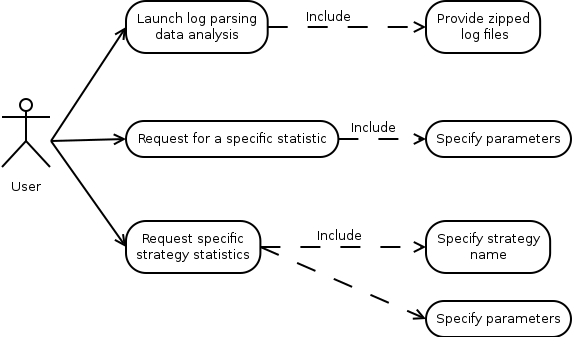
\includegraphics[width=\textwidth,height=\textheight,keepaspectratio]{UseCaseParsing}
% \newpage
% \textbf{this image shows with more details the use-case of the data analyzes and
% data recovery.}\\
% \\
% 
\includegraphics[width=\textwidth,height=\textheight,keepaspectratio]{UseCaseDataMining}

% \newpage
% 
\includegraphics[width=\textwidth,height=\textheight,keepaspectratio]{UseCaseParser}
\section{User interface}
The program user interface will be composed of a executable(dominionmining) that will be
executed with certain parameters to execute the desired action.
The following diagram represents the different interactions available to the user:\\
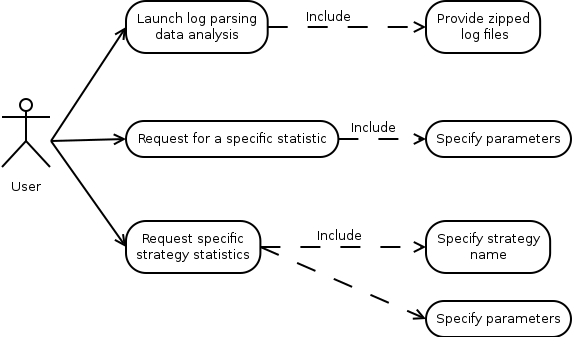
\includegraphics[scale=0.45,keepaspectratio]{UseCaseParsing}\\
Before the use of any features of the program , the user has to launch the parsing.
\subsection{Launching the log parsing}
\subsubsection{Description and Priority}
\textbf{Priority level=high}\\
\begin{itemize}
  \item The user will have to place all the compressed logs (tar.bz2 files) to be parsed into a
    specific folder.
  \item Once the previous step is done, the user can execute the parsing by
      typing : \textit{dominionmining parse (zlib/snappy)} if no compression is
      given the default compression is \textit{snappy}.
    %TODO \item For testing purposes, in order to avoid having a 4 hours parsing step, the user can specify a percentage of the logs to be parsed. by specifing a value between 0 and 100. the parser will randomly select logs from the provided ones and parse them, creating a usable database for further testing.
    \item once the parsing is done a message will be shown on the
      console (parsing done).
\end{itemize}

%TODO
%\subsection{Game data mapping}
%In order to allow the user to ask for specific statistics concerning a game, the program can be run in order to generate simplified game logs and then a python script will be applied to this log. This would allow more flexibility in the type of statistics displayable by the program.
%\begin{itemize}
%\item the program will be launched by using the following command: \textit{dominionmining data\_to\_query user\_script.py}
% \item the python script will be applied to the generated result and return the statistics asked by the user.
%\item The generated file containing the query results will have the following format:
%\begin{itemize}
%\item The name of the produced file is \textit{game.txt}
%\item The simplified log will contain each action made by the player, one action per line(TODO: provide a list of actions and their name in the simplified log). List of actions and their format:
%\begin{itemize}
%\item Revealing a card: \textit{player\_x reveals card\_name}
%\item Drawing cards: \textit{player\_x draws n cards}
%\item Buying a card: \textit{player\_x buys card\_name}
%\item Trashing cards: \textit{player\_x trashes n cards}
%\item Puts a card: \textit{player\_x puts card\_name}
%\item Gaining a card: \textit{player\_x gains card\_name}
%\item Plays a card: \textit{player\_x plays card\_name}
%\end{itemize}
%\end{itemize}
%\end{itemize}

\subsection{Statistics requests}
\subsubsection{Description and Priority}
\textbf{Priority level=high}\\
The request for a statistic can be made by typing \textit{dominionmining stats (parameters)}.  \\
The possible strategy names are:
bigmoney , penprovince , beyondsilver.\\
If other strategies are recognized by the program they will be added to the list.\\
The list of parameters that will be possible to use will be determined in the
future.\\

The return of a statistic can be a chart displayed in a window or exported to a
file. If its a single value, a name or a sentence it will be returned in the prompt.

\section{Data Modeling}

\subsection{Log decompression}
\subsubsection{Description and Priority}
\textbf{Priority level=high}\\


\begin{itemize}
  \item The tar.bz2 files will be stored in a folder.
  \item The program will decompress one specified file from this folder in a temporary folder.
  \item The programm will delete the decompressed logs on demand by the parser.
\end{itemize}

\subsection{Parser}

\subsubsection{Description and Priority}

\textbf{Priority level=high}\\

Provided the issues revealed by the logs (like: the inconsistency of the syntax)
a use of a parser made with tools like \textit{YACC and LEX} is not recommended.
For that a parser will be done by using the already present \textit{HTML} and
key words presents on the logs.\\
The parser is responsible for reading the logs and collecting the important
information without losing the structure of the log.\\
A glimpse of the data to be recognized by the parser is illustrated in this
diagram (some data to be determined as all the possibilities inside a log
haven't been revealed yet):\\

\includegraphics[scale=0.35,keepaspectratio]{UseCaseParser}

\begin{itemize}
\item Winners: The list of the winners of the game, it can be one winner or several winners if they are tied.
\item Market: The list of 10 available cards to be bought by the players.
\item Cards Gone: list of cards that have been entirely bought at the end of the game.
\item Player Name: Name of the player.
\item Victory points: Amount of points at the end of the game.
\item Player cards: List of cards bought by the player with the amount they bought.
\item Victory cards: List of victory cards the player with the bought.
\item Trash: List of cards that that are discarded at the end of the game.
\item Game Moves: Every action depending on this item correspond to an action performed during a player's turn.
\end{itemize}

The parser has to read every element shown in the previous graph as a part of the data when the user launches the parsing process.\\


\subsection{Create game-log}
\subsubsection{Description and Priority}
\textbf{Priority level=high}\\
This functionality is the creation of a data structure where the log data will
be remodeled into.
here is a graphical representation of an overview of the data structure:\\
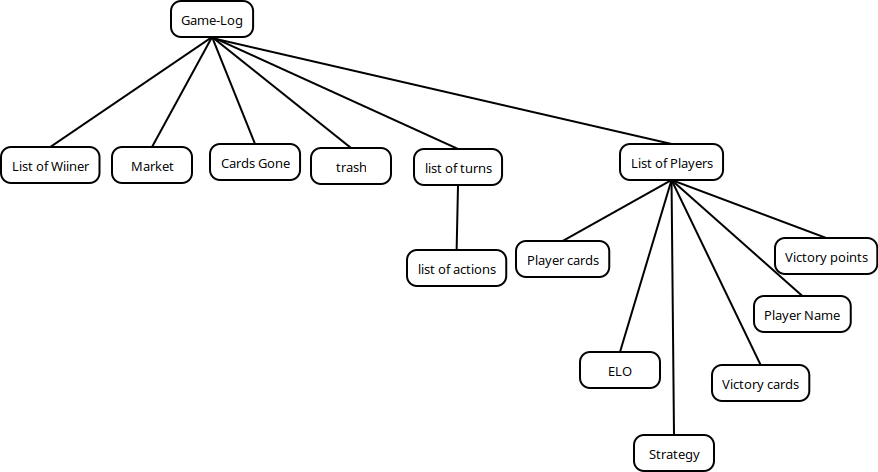
\includegraphics[scale=0.5,keepaspectratio]{game-log}

\subsection{Send game-log data}
\subsubsection{Description and Priority}
\textbf{Priority level=high}\\
The program will send the game-log data structure to the database part of the project.
\section{Data Storage}


\subsection{Connect to Relational Database}
\subsubsection{Description and Priority}
\textbf{Priority level=high}\\
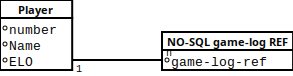
\includegraphics[keepaspectratio]{SQL}
\begin{itemize}
\item The program will be able to send data relative to the player (eg: ID, Name, Elo, Games played by the player)
\item The program will be able to send requests to the database concerning every piece of data stored in it.
\item The relational database will send the results of the requests made by the program.
\end{itemize}


\subsection{Create document-oriented Database}

\subsubsection{Description and Priority}
\textbf{Priority level=high}\\
This module will be responsible to create the document-oriented database containing data at the JSon format.

\subsection{Connect to document-oriented Database}
\subsubsection{Description and Priority}
\textbf{Priority level=high}\\
\begin{itemize}
\item The document-oriented database will be handling exchanges through a specific socket.
\item The document-oriented database will receive game-logs at the JSon format.
\item The document-oriented database will receive requests from the program concerning every piece of data contained in it.
\item The document-oriented database will send results of the requests made by the program.
\end{itemize}


\subsection{Compression}
\subsubsection{Description and Priority}
\textbf{Priority level=medium}\\
The document-oriented database will hold most of the data and some level of compression
will have to be applied.
The database in focus to be used at the moment is \textit{mongodb} and it offers
2 levels of compression \textit{Zlib} and \textit{Snappy}.
During the development the \textit{Snappy} will be used as it offers a better
performance.
But the final program should give the user the ability to chose the compression
level when starting the log parsing.


\subsection{Save game-log}
\subsubsection{Description and Priority}
\textbf{Priority level=high}\\
\begin{itemize}
\item The document-oriented database will convert the game-log structure in a JSon formatted document.
\item The produced data in JSon format will be stored in the database.
\end{itemize}

\subsection{Load game-log}
\subsubsection{Description and Priority}
\textbf{Priority level=high}\\
When asked for a game-log, the database will load the JSon formatted log in a game-log data structure indetical to the one described in the data modelling section.\\
If there is missing information in the JSon document, the corresponding field will be left empty.



\section{Data Analysis}

\subsection{Gather data}
\subsubsection{Description and Priority}
\textbf{Priority level=high}\\
\begin{itemize}
\item The data analyser will convert the query results in a format usable by the plotting module.
\item If the data is simple to read (eg: a number, a name, a sentence), the data analyser will simply output the result in text format.
\item The last query will be memorized with it's result in order to gain time if the next query made by the user is the same.
\item If the user wants to apply a python script to game logs, the pogram will request the game logs and put them in a text file, this file will contain each action made by each player and the script will be applied to this file.
\end{itemize}

\subsection{restore game-log}
\subsubsection{Description and Priority}
\textbf{Priority level=medium}\\
This feature is responsible to restore the missing information on the parsed
logs, by using deduction based on the data obtained from the log.\\
In case of a missing game header or part of it missing:
  \begin{itemize}
  \item Winners/victory cards/victory points missing: the program can keep track of the cards owned by the players during the game in order to know how many victory cards they have at the end of the game.
  \item Market missing: The program can keep track of the cards bought during the game in order to partially or totally reconstruct the cards available in the Market.
  \item Cards Gone: As with a missing Market data, the program will keep track of cards bought and count the amount bought for each card, if the maximum amount of cards is bought, the card is gone at the end of the game.
  \item Player name missing: the game moves part of a log also keeps track of the player names, the program will simply restore them in the header.
  \item Player cards: the program will keep track of the actions performed during the game relative to the player cards and add them in this list.
  \end{itemize}

\subsection{Plotting}
\subsubsection{Description and Priority}
\textbf{Priority level=high}\\
The plotting module will get the converted data obtained after the Gather Data process and will plot them in a graphical interface. This module will work in a similar way of \textit{GnuPlot}.

\subsection{Calculate \textit{\textbf{ELO}}}
\subsubsection{Description and Priority}
\textbf{Priority level=high}\\
The analyzer will have to calculate the final ELO for each player and what was a
player ELO on a given game.
For each game in chronological order, this module will request the initial elo of the players from the relational database and the winners of the game, then it will calculate the new elo of each player from the outcome of the game. The module will then set the calculated elo in the document-oriented database at the currently analyzed game and will also update the overall elo for each of the players participating in the game on the relational database.\\
More information about ELO can be found on \url{https://en.wikipedia.org/wiki/Elo_rating_system}\\
The following diagram illustrates the process of the elo calculation:\\
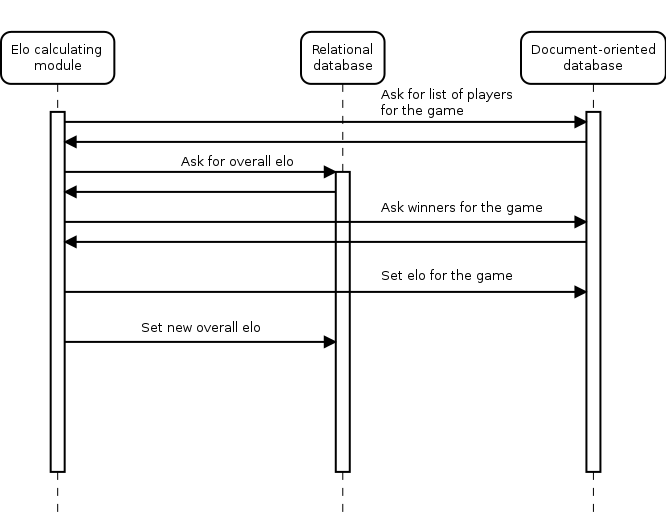
\includegraphics[width=\textwidth,height=\textheight,keepaspectratio]{elocalc}\\

\subsection{Recognize strategies}
\subsubsection{Description and Priority}
\textbf{Priority level=medium}\\

The dominion wiki describes some strategies that can be used in the game .\\ For exemple :\\
Big Money\\
Beyond Silver \\
Penultimate Province Rule \\
More on \url{http://wiki.dominionstrategy.com/index.php/Strategy}\\

And the analyzer will have to be able to recognize what strategy was used on a
given match (if any strategy was used) and generate statistics.\\
\textbf{This image describes the decision process involved in the Big Money strategy}\\
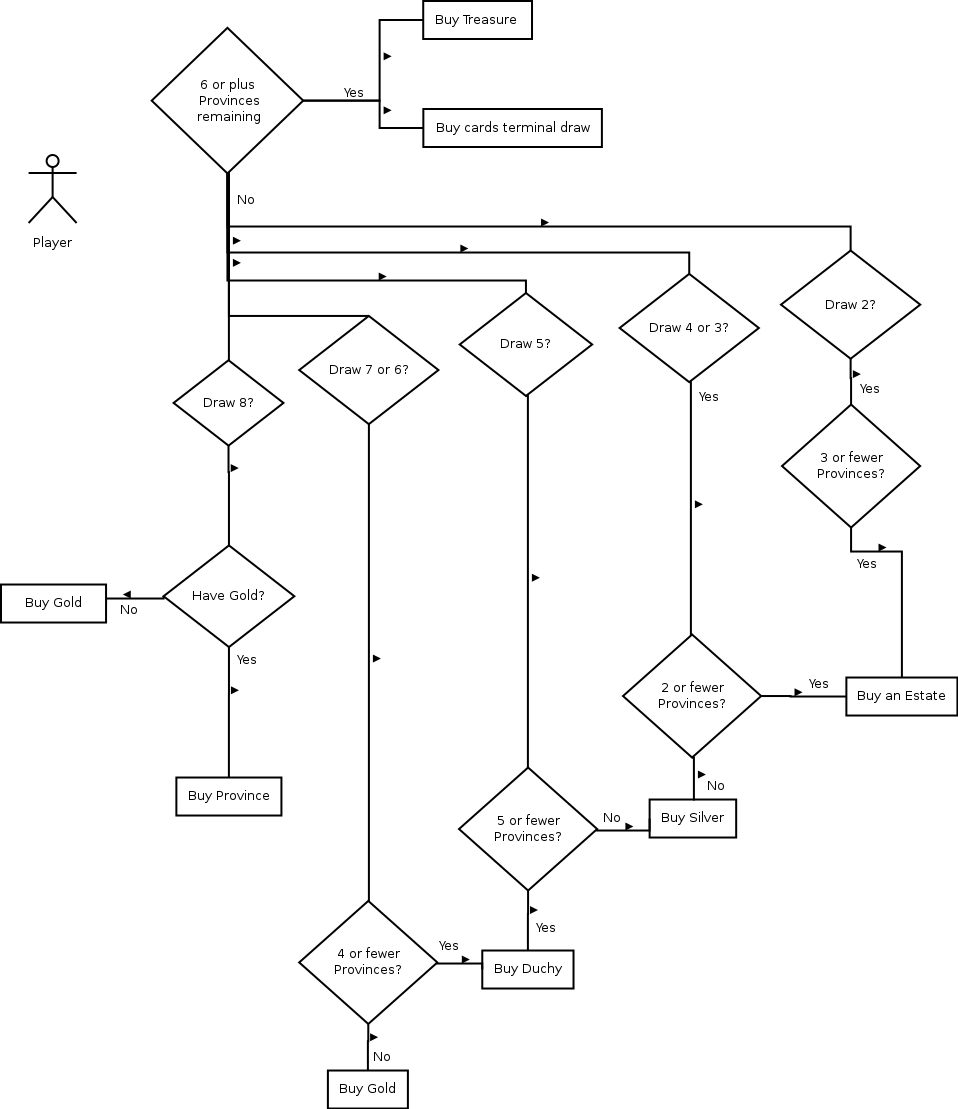
\includegraphics[width=\textwidth,height=\textheight,keepaspectratio]{big-money}\\
The analyzer has to recognize when a player buys only money cards and specific cards related to the big money strategy. It also has to keep track of the remaining provinces to be bought.\\
More on \url{http://wiki.dominionstrategy.com/index.php/Big_Money}\\

In order to recognize the strategy coined Beyond Silver, the analyzer has to recognize when certain type of cards are bought, the list of these cards can be found on \url{http://wiki.dominionstrategy.com/index.php/Silver#Beyond_Silver}\\

In order to recognize that the Penultimate Province Rule is respected (as explained on \url{http://dominionstrategy.com/2011/03/28/the-penultimate-province-rule/}), the analyzer has to keep track of the amount of Victory Points of each player at every turn.

\subsection{Recognize Greening}
\subsubsection{Description and Priority}
\textbf{Priority level=high}\\
The analyzer has to be capable of recognize the \textit{\textbf{greening}} moment on each match.
More about \textit{\textbf{greening}} on \url{http://wiki.dominionstrategy.com/index.php/Greening}.\\
The program will recognize when the greening happens by detecting when victory cards begin to be bought.


\chapter{Nonfunctional Requirements}

\section{Performance Requirements}
% $<$If there are performance requirements for the product under various
% circumstances, state them here and explain their rationale, to help the
% developers understand the intent and make suitable design choices. Specify the
% timing relationships for real time systems. Make such requirements as specific
% as possible. You may need to state performance requirements for individual
% functional requirements or features.$>$
No specific performance requirement was made by the client. But for the analyzer
a time of running should be less than an hour.\\
%TODO: peut-etre a précisier
The user should be able to iterate the analysis process on a precise dataset without having to wait for the same query to be done again.



\section{Reliability}
The client demands that the maximum number of logs should be parsed , as the
data provided has some inconsistencies and some logs wont be possible to parse.
the client agrees that between 5 to 10\% of the logs can be ignored.\\

The parser will have to parse 100\% of the data present on the log and Restore
any missing information if possible.\\

\section{Software Quality Attributes}
% $<$Specify any additional quality characteristics for the product that will be
% important to either the customers or the developers. Some to consider are:
% adaptability, availability, correctness, flexibility, interoperability,
% maintainability, portability, reliability, reusability, robustness, testability,
% and usability. Write these to be specific, quantitative, and verifiable when
% possible. At the least, clarify the relative preferences for various attributes,
% such as ease of use over ease of learning.$>$
Even if just a command line is expected for the final program it should have a
easy learn curve and be easy to use.\\
The data generated by the parser don't need to be human readable.\\
%TODO: The game logs generated will have to be analyzeable by the user in order to allow as much flexiblity as possible in the treatment of the logs.


%\chapter{Other Requirements}
% $<$Define any other requirements not covered elsewhere in the SRS. This might
% include database requirements, internationalization requirements, legal
% requirements, reuse objectives for the project, and so on. Add any new sections
% that are pertinent to the project.$>$

%\section{Appendix A: Glossary}
% %see https://en.wikibooks.org/wiki/LaTeX/Glossary
% $<$Define all the terms necessary to properly interpret the SRS, including
% acronyms and abbreviations. You may wish to build a separate glossary that spans
% multiple projects or the entire organization, and just include terms specific to
% a single project in each SRS.$>$

%\section{Appendix B: Analysis Models}
% $<$Optionally, include any pertinent analysis models, such as data flow
% diagrams, class diagrams, state-transition diagrams, or entity-relationship
% diagrams.$>$

%\section{Appendix C: To Be Determined List}
% $<$Collect a numbered list of the TBD (to be determined) references that remain
% in the SRS so they can be tracked to closure.$>$

\end{document}
